%\newcommand{\DIR}{DIR = /}
	

\subsection{Amostragem} 

\textbf{\textit{\\Conceitos}} 

\textbf{\textit{\\População}}: Alvo do estudo.
\textbf{\textit{\\\\Censo}}: Pesquisa com toda a população, pode ser caro ou impossível inferir sobre toda a população.
\textbf{\textit{\\\\Enviesamento}}: Você subestima ou superestima o parâmetro da população. 
\textit{causas}: Pesquisa de pessoas próximas ou de fácil acesso, pesquisas pela internet, sem uso de mecanismo de seleção aleatório.

\textbf{\textit{\\Amostra}} - Parte de uma população (Subconjunto da população), selecionada usando alguma técnica que de chances iguais a todos os elementos da população de serem selecionados. 
\\\\Uma amostra feita corretamente deve representar as mesmas características da população de onde foi retirada.
\\\\Se ela não representa a população, dizemos que ela é enviesada.
\textbf{\\\\"Custo" da Amostra}
\\Margem de erro e nível de confiança.
\\Variação: amostrar diferentes podem apresentar resultados diferentes.
\\podemos "medir" a variação esperada.

\newpage

\textbf{\textit{\\Principais tipos de amostras}} 

\textbf{\textit{\\Aleatória simples - }}
Um determinado número de elementos é retirado da população de forma aleatória.
Todos os elementos da população alvo do processo de amostragem, devem ter as mesmas chances 
de serem selecionado para fazer parte da amostra.


{\centering 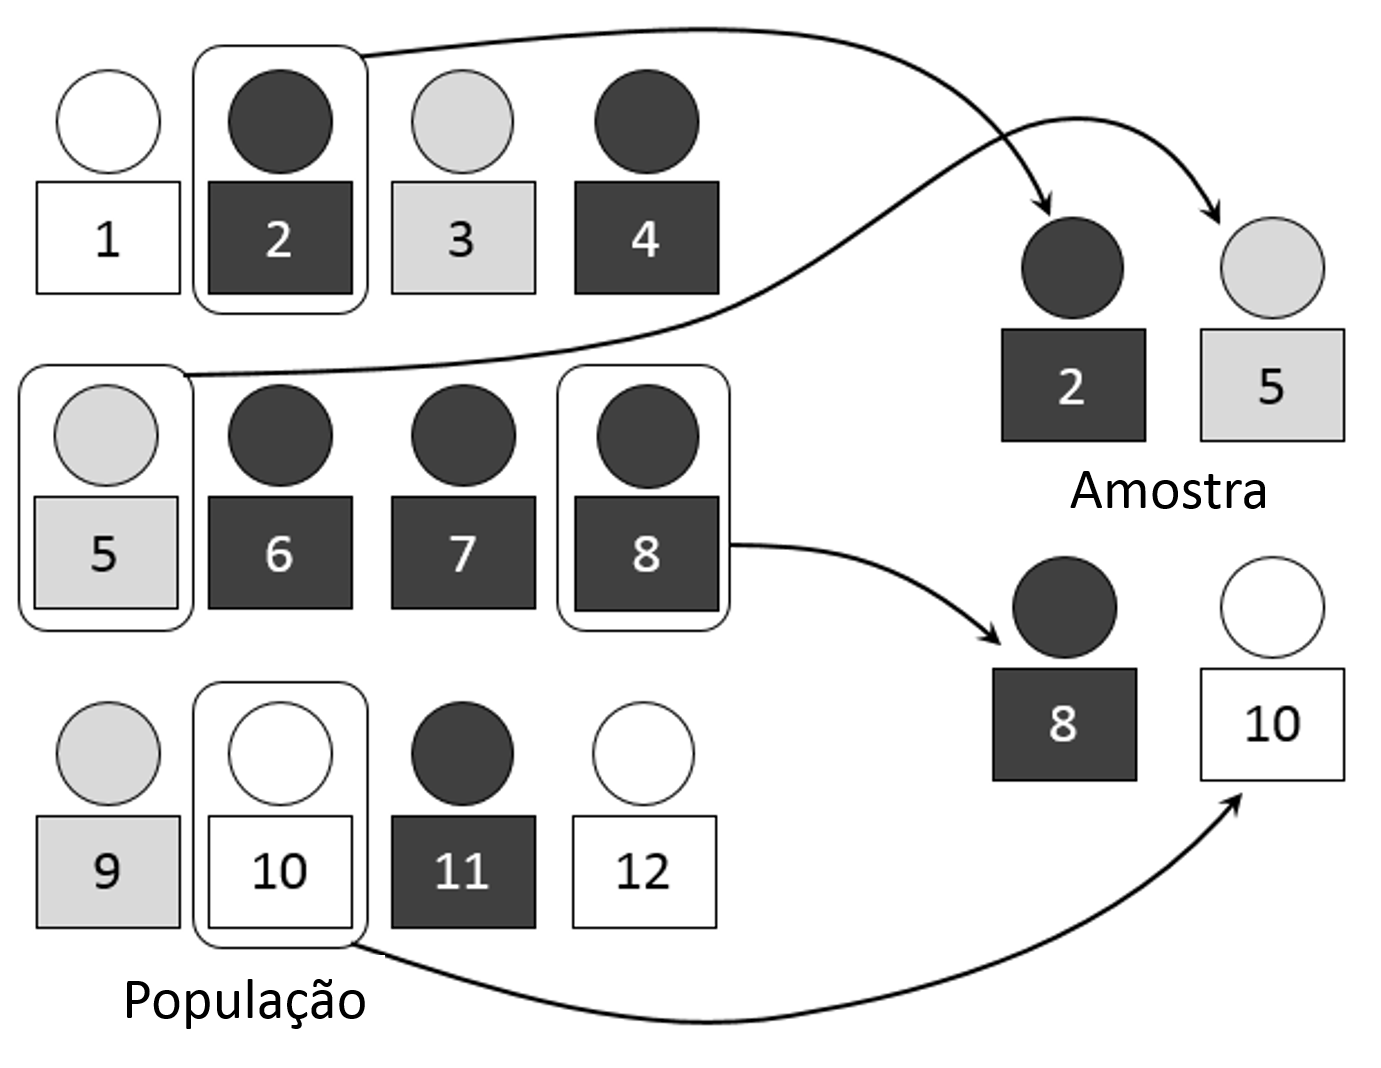
\includegraphics[scale=0.17]{cap1/Amostragem/AleatoriaSimples.png} \par}

Há duas formas de trabalhar com amostra aleatória simples, com reposição e sem reposição. 

\textit{Com reposição:}
Quer dizer que uma vez que o elemento da população é selecionado, ele volta a fazer parte da população 
e ele passa a ter as mesmas chances de ser selecionado novamente, exemplo(Exame de dopping em atletas das olimpíadas). 

{\centering 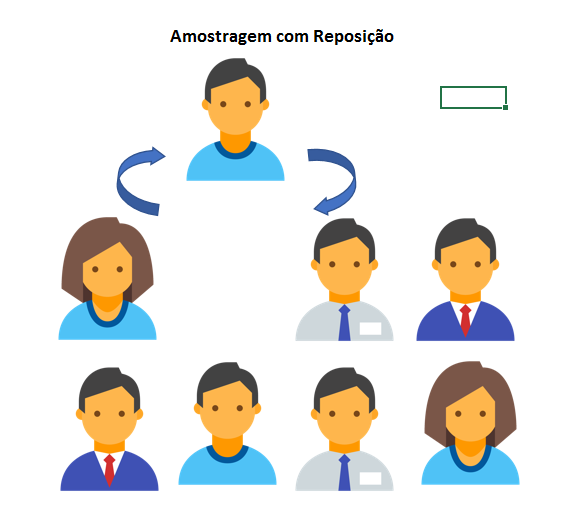
\includegraphics[scale=0.45]{cap1/Amostragem/amostragemComReposicao.png} \par}

\newpage

\textit{Sem reposição:}
Uma vez que o elemento da população é selecionado, ele não faz mas parte da população e não tem mais chance ser selecionado novamente, exemplo(Pesquisa de intensão de votos). 

{\centering 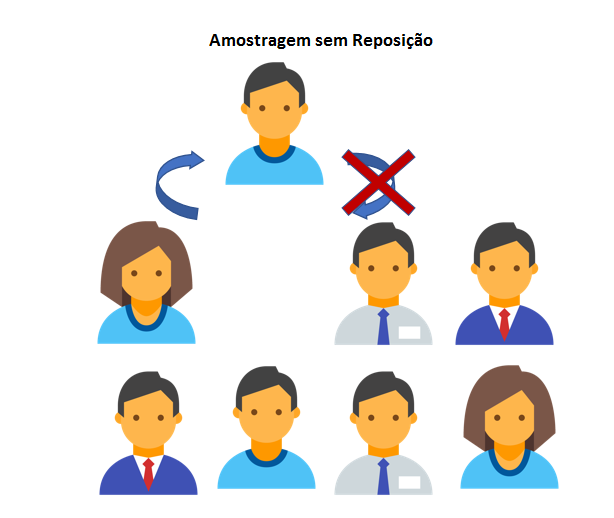
\includegraphics[scale=0.45]{cap1/Amostragem/amostragemSemReposicao.png} \par}

\textbf{\textit{\\Estratificada -}}
As vezes as populações estão divididas nos chamados estratos, características comuns que os elementos tem, podem ser relacionados a raça, escolaridade ou religião.

{\centering 
\includegraphics[scale=0.45]{cap1/Amostragem/amostragemEstratificada.jpg} \par}

\textbf{\textit{\\Sistemática -}}
Neste tipo de amostragem, é escolhido um elemento aleatório, e a partir daí, a cada N elementos um novo membro é escolhido.

{\centering 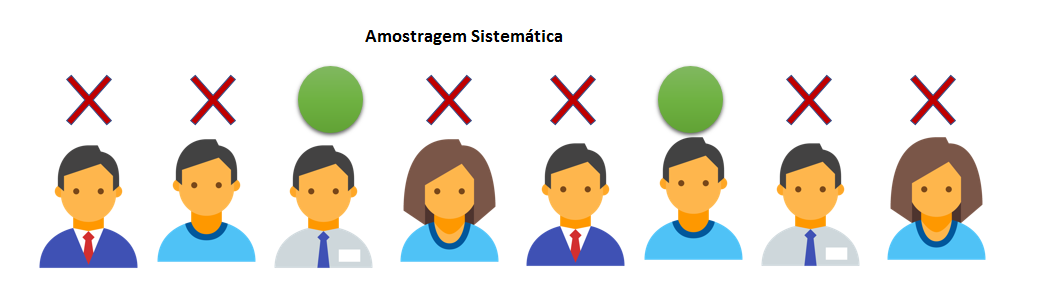
\includegraphics[scale=0.45]{cap1/Amostragem/amostragemSistematica.png} \par}

\newpage

\textbf{\textit{\\Por Unidade Monetária -}}
Neste tipo de amostra é informada uma coluna de ordenação, e uma coluna numérica que sera utilizada 
para gerar os cálculos para produzir a amostra.

{\centering 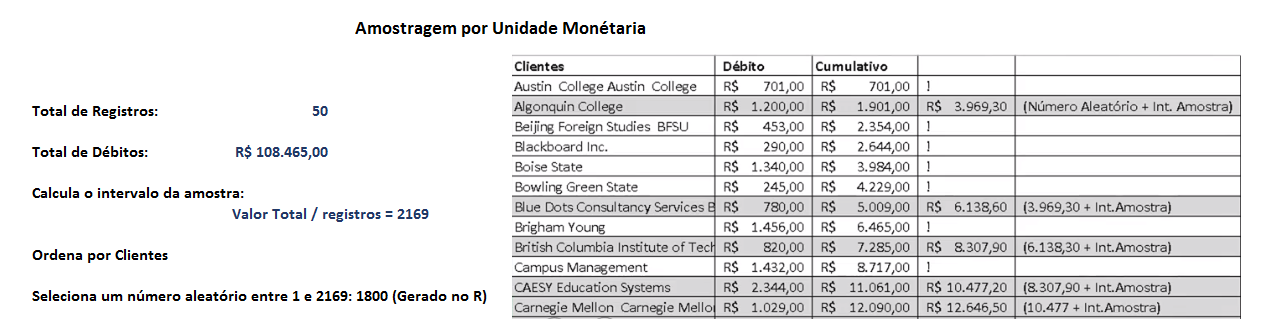
\includegraphics[scale=0.45]{cap1/Amostragem/amostragemPorUnidadeMonetaria.png} \par}

\newpage

\subsection{Amostragem - R} 

\subsubsection{Aleatória simples}

Utilizando o R vamos demonstrar a amostragem utilizando o dataset Iris.
Mais informações sobre o dataset: \href{https://en.wikipedia.org/wiki/Iris_flower_data_set}{dataset iris}
\\\\bibliotecas que devem ser importadas:
\\\newline{library(datasets) - importa os Datasets}
\newline{data(iris) - importa o Dataset Iris} 
\newline{summary(iris) - produz o resultado sumarizado do dataset}
\newline{dim(iris) - Retorna o conjunto da dimensão de um objeto}
\\\\Para o exemplo vamos criar um modelo separando os dados do dataset IRIS em dois conjuntos.
\textbf{\textit{\\Passos}}
\\1 - Gerar 150 números aleatórios, que poderão ser 0 ou 1 gerar 150 números aleatórios.
\\2 - Usar esses números aleatórios e dividi-los por números aleatórios.
\\\\Função sample é composta por 4 parametros, onde o primeiro parametro indica de onde ele vai buscar a amostra, 
neste caso ele ira escolher apenas 0 ou 1, o segundo parametro indica o tamanho da amostra, o terceiro(replace) 
indica que sera uma amostra com reposição e por ultimo o vetor de probabilidade indicando q cada numero tera 50% 
de chance de ser escolhido.
\\

{\centering 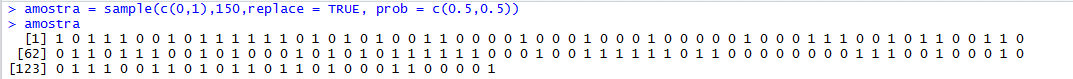
\includegraphics[scale=0.50]{cap1/Amostragem/AleatoriaSimplesR.png} \par}

\newpage
\textbf{Total da amostra}
\\\\Total da Amostra que é igual a 1
\\length(amostra[amostra==1])
\\\\Total da Amostra que é igual a 0
\\length(amostra[amostra==0]
\\

	\begin{figure}[h!]
    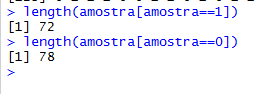
\includegraphics[scale=1.0]{cap1/Amostragem/AleatoriaSimplesRAmostraLength.png} 
	\end{figure}


\textbf{Repetir um experimento}
\\Cria uma semente de aleatoriedade que permite repetir o experimento.
\\set.seed(2345)
\\sample(c(100),1)

	\begin{figure}[h!]
	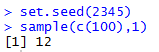
\includegraphics[scale=1.0]{cap1/Amostragem/AleatoriaSimplesRAmostraSeed.png} 
	\end{figure}

\newpage

\subsubsection{Estratificada}

Para gerar uma amostra estratificada, vamos utilizar o Dataset iris.

O comando summary mostra as informações do Dataset de forma sumarizada\\. 

{\centering 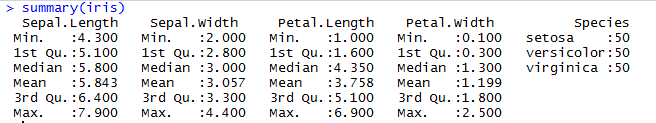
\includegraphics[scale=0.8]{cap1/Amostragem/amostragemEstratificadaR.png} \par}

Será necessário instalar o pacote sampling(Função para desenhos e calibração de amostras.)
\href{https://cran.r-project.org/web/packages/sampling/index.html}{Package sampling}
\\\\
Carregar o pacote na memória.
\\library(sampling)
\\\\
Gerar Estrato 
\\
Função strata : primeiro passa-se o conjunto de dados depois o vetor com as 
colunas(neste caso vamos utilizar apenas uma coluna(species)), e por fim o vetor 
com o tamanho de cada estrato.
\\\\
amostrairis2 = strata(iris, c("Species"), size=c(25,25,25), method="srswor")\\

{\centering 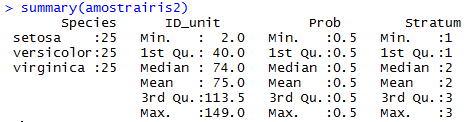
\includegraphics[scale=1.0]{cap1/Amostragem/amostragemEstratificadaR2.png} \par}

\newpage

Caso desejarmos gerar uma amostra estratificada em que haja uma proporção de elementos. 
para isso utilizaremos o Dataset Infert.\\

{\centering 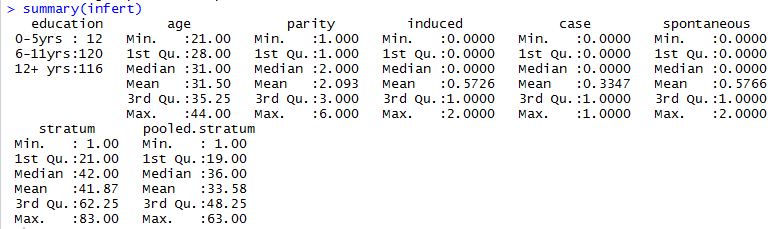
\includegraphics[scale=0.7]{cap1/Amostragem/amostragemEstratificadaR2Infert.png} \par}

Precisamos gerar uma amostra com 100 elementos, portanto precisamos calcular o numero de elementos do estrato dividido pela população versus o tamanho da amostra.
\\\\
Entre 6 e 11 anos temos 120.
\\
length(infert[infert=='6-11yrs'])\\

{\centering 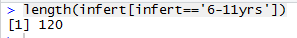
\includegraphics[scale=1.0]{cap1/Amostragem/amostragemEstratificadaR2Infert2.png} \par}


Numero de elementos do Dataset.
\\
length(infert\$education)\\

{\centering 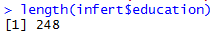
\includegraphics[scale=1.0]{cap1/Amostragem/amostragemEstratificadaR2Infert3.png} \par}

Tamanho da amostra que desejo gerar.
\\100\\

Cálculo.
\\
\textbf{\textit{120 / 248 * 100}}

{\centering 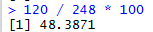
\includegraphics[scale=1.0]{cap1/Amostragem/amostragemEstratificadaR2Infert4.png} \par}

\newpage

Resultados
\\unique(infert\$education)
\\round(length(infert[infert=='0-5yrs'])/length(infert\$education)*100)
\\round(length(infert[infert=='6-11yrs'])/length(infert\$education)*100)
\\round(length(infert[infert=='12+ yrs'])/length(infert\$education)*100)\\

{\centering 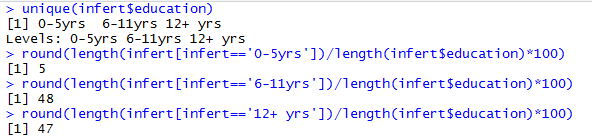
\includegraphics[scale=0.8]{cap1/Amostragem/amostragemEstratificadaR2Infert5.png} \par}

Utilizando a função strata.
\\'0-5yrs' = round(length(infert[infert=='0-5yrs'])/length(infert\$education)*100)
\\'6-11yrs' = round(length(infert[infert=='6-11yrs'])/length(infert\$education)*100)
\\'12+ yrs' = round(length(infert[infert=='12+ yrs'])/length(infert\$education)*100)
\\amostra = strata(infert, c("education"), size=c(`0-5yrs`,`6-11yrs`,`12+ yrs`), method="srswor")
\\summary(amostra)\\

{\centering 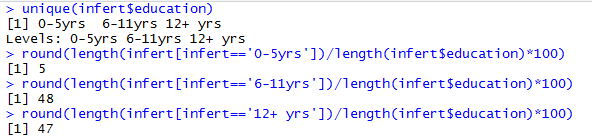
\includegraphics[scale=0.8]{cap1/Amostragem/amostragemEstratificadaR2Infert5.png} \par}

O método srswor - método padrão da função strata que gera uma amostra aleatória sem reposição

\newpage

\subsubsection{Sistemática}

Para estudarmos a amostragem sistemática, precisamos  instalar o pacote TeachingSampling.
\\install.packages("TeachingSampling")
\\Depois carregar o pacote na memória.
\\library(TeachingSampling)
\\\\TeachingSampling vai gerar números aleatórios que poderão ser utilizados pra fazer a amostra, então vamos gerar uma amostragem aleatória sistemática no conjunto de dados iris 
e essa amostra sistemática pega uma instancia do conjunto de dados iris a cada dez.
\\\\Vai gerar uma um numero aleatório a cada dez registros.
\\amostra = S.SY(150, 10) \\

{\centering 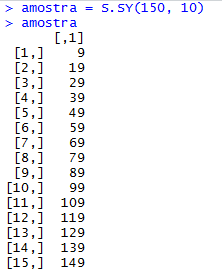
\includegraphics[scale=0.8]{cap1/Amostragem/amostragemSistematicaR1.png} \par}

Utilizando a amostra para selecionar os dados do Dataset Iris.\\

 {\centering 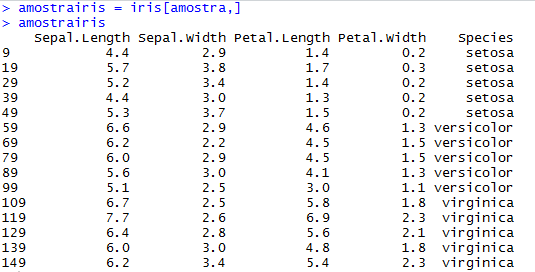
\includegraphics[scale=0.8]{cap1/Amostragem/amostragemSistematicaR2.png} \par}
